%%
%% This is file `sample-manuscript.tex',
%% generated with the docstrip utility.
%%
%% The original source files were:
%%
%% samples.dtx  (with options: `manuscript')
%% 
%% IMPORTANT NOTICE:
%% 
%% For the copyright see the source file.
%% 
%% Any modified versions of this file must be renamed
%% with new filenames distinct from sample-manuscript.tex.
%% 
%% For distribution of the original source see the terms
%% for copying and modification in the file samples.dtx.
%% 
%% This generated file may be distributed as long as the
%% original source files, as listed above, are part of the
%% same distribution. (The sources need not necessarily be
%% in the same archive or directory.)
%%
%% The first command in your LaTeX source must be the \documentclass command.
%%%% Small single column format, used for CIE, CSUR, DTRAP, JACM, JDIQ, JEA, JERIC, JETC, PACMCGIT, TAAS, TACCESS, TACO, TALG, TALLIP (formerly TALIP), TCPS, TDSCI, TEAC, TECS, TELO, THRI, TIIS, TIOT, TISSEC, TIST, TKDD, TMIS, TOCE, TOCHI, TOCL, TOCS, TOCT, TODAES, TODS, TOIS, TOIT, TOMACS, TOMM (formerly TOMCCAP), TOMPECS, TOMS, TOPC, TOPLAS, TOPS, TOS, TOSEM, TOSN, TQC, TRETS, TSAS, TSC, TSLP, TWEB.
% \documentclass[acmsmall]{acmart}

%%%% Large single column format, used for IMWUT, JOCCH, PACMPL, POMACS, TAP, PACMHCI
% \documentclass[acmlarge,screen]{acmart}

%%%% Large double column format, used for TOG
% \documentclass[acmtog, authorversion]{acmart}

%%%% Generic manuscript mode, required for submission
%%%% and peer review
%\documentclass[manuscript,screen,review]{acmart}
\documentclass[sigconf,review]{acmart}


%% Fonts used in the template cannot be substituted; margin 
%% adjustments are not allowed.
%%
%% \BibTeX command to typeset BibTeX logo in the docs
\AtBeginDocument{%
 \providecommand\BibTeX{{%
   \normalfont B\kern-0.5em{\scshape i\kern-0.25em b}\kern-0.8em\TeX}}}
    
  %  \AtBeginDocument{\renewcommand*{\thesubfigure}{\alphalph{\value{subfigure}}}}

%% Rights management information.  This information is sent to you
%% when you complete the rights form.  These commands have SAMPLE
%% values in them; it is your responsibility as an author to replace
%% the commands and values with those provided to you when you
%% complete the rights form.


\setcopyright{none} % remove permission section
\settopmatter{printacmref=false} % remove ACM reference format
\renewcommand\footnotetextcopyrightpermission[1]{} % removes footnote with conference information in first column
\pagestyle{plain}
%\setcopyright{acmcopyright}
%\copyrightyear{2022}
%\acmYear{2022}
%\acmDOI{00.0000/0000000.0000000}

%% These commands are for a PROCEEDINGS abstract or paper.
%\acmConference[Woodstock '18]{Woodstock '18: ACM Symposium on Neural Gaze Detection}{June 03--05, 2018}{Woodstock, NY}
  \acmConference[SSW625 Phase 3]
{SSW625 Group Project -- Phase 3}
{November 9, 2026}
{Stevens Institute of Technology}
\acmBooktitle{MSR '22: Proceedings of the 19th International Conference on Mining Software Repositories, May 23–24, 2022, Pittsburgh, PA, USA}
\acmPrice{15.00}
\acmISBN{978-1-4503-XXXX-X/18/06}

\usepackage{xspace}
\newcommand{\ie}{\textit{i.e.}}
\newcommand{\eg}{\textit{e.g.}}
\newcommand{\etal}{\textit{et al. \xspace}}
%\usepackage{array}
%\newcolumntype{L}{>{\arraybackslash}m{8cm}}
%%%%% Long text wrap %%%%%
\usepackage{array}
\newcolumntype{L}{>{\arraybackslash}m{16cm}}
%\newcolumntype{L}[1]{>{\raggedright\let\newline\\arraybackslash\hspace{0pt}}m{#1}}
\newcolumntype{C}[1]{>{\centering\let\newline\\arraybackslash\hspace{0pt}}m{#1}}
\newcolumntype{R}[1]{>{\raggedleft\let\newline\\arraybackslash\hspace{0pt}}m{#1}}
%%%%% Long text wrap %%%%%
%\usepackage{adjustbox}
%\usepackage{subcaption}
%\usepackage{textcomp}
%\usepackage{pgfplots}
\usepackage[numbered]{bookmark}
%\usepackage{soul}
%\usepackage{booktabs}
%\usepackage{multirow}
%\usepackage{float}
%\usepackage{url}
\usepackage{tcolorbox}
\usepackage{graphicx}
%\usepackage{textcomp}
\usepackage{xcolor}
%\usepackage{url}
\usepackage{tabularx} 
%\usepackage{balance}
\usepackage{stfloats}
%\usepackage{fullpage}
\usepackage[justification=centering]{caption}
\usepackage{lineno}
\usepackage[title]{appendix}
\usepackage{dirtytalk}
\usepackage{amsmath}
%\usepackage{tikz}
\usepackage{pgfplots, pgfplotstable}
%\usetikzlibrary{tikzmark}
\usetikzlibrary{patterns}



%%%%%
%-----------------------
%\usepackage[utf8]{inputenc}
\usepackage[english]{babel}
%\usepackage{amssymb}
\usepackage{textcomp}
%\usepackage{indentfirst}
%\setcounter{tocdepth}{3}
\usepackage{mathtools}
%\usepackage[usestackEOL]{stackengine}
%\usepackage{amsmath}
\usepackage{ltxtable}
\usepackage{algorithm}
\usepackage{algpseudocode}
\usepackage{textcomp}
%\usepackage{mathpazo}
%\usepackage{tgpagella}
%-----------------------

\usepackage{tcolorbox}

%\usepackage[dvipsnames]{xcolor}
\usepackage{pgf-pie}
%\usepackage{pgfplots}
%\pgfplotsset{compat=1.14}
%%%%%%%%%%%%%%%%%%%%%%%%%%%%%%%%%%%%%%%%%%%%%%%%%%%
\definecolor{wedge1}{RGB}{ 190  30  46}
\definecolor{wedge2}{RGB}{ 240  65  54}
\definecolor{wedge3}{RGB}{ 241  90  43}
\definecolor{wedge4}{RGB}{ 247 148  30}
\definecolor{wedge5}{RGB}{  43  56 144}
\definecolor{wedge6}{RGB}{  28 117 188}
\definecolor{wedge7}{RGB}{  40 170 225}
\definecolor{wedge8}{RGB}{ 119 179 225}
\definecolor{wedge9}{RGB}{ 181 212 239}
\definecolor{wedge10}{RGB}{  0 104  56}
\definecolor{wedge11}{RGB}{  0 148  69}
\definecolor{wedge12}{RGB}{ 57 181  74}
\definecolor{wedge13}{RGB}{141 199  63}
\definecolor{wedge14}{RGB}{215 244  34}
\definecolor{wedge15}{RGB}{249 237  50}
\definecolor{wedge16}{RGB}{248 241 148}
\definecolor{wedge17}{RGB}{242 245 205}
\definecolor{wedge18}{RGB}{123  82  49}
\definecolor{wedge19}{RGB}{104  73 158}
\definecolor{wedge20}{RGB}{102  45 145}
\definecolor{wedge21}{RGB}{148 149 151}
\definecolor{wedge22}{RGB}{ 204 50 153}
\definecolor{wedge23}{RGB}{ 79 47 79}
\definecolor{wedge24}{RGB}{ 173 234 234}
\definecolor{wedge25}{RGB}{ 216 191 216}
\definecolor{wedge26}{RGB}{  43  56 144}
\definecolor{wedge27}{RGB}{  40 170 225}
\definecolor{wedge28}{RGB}{ 119 179 225}
\definecolor{wedge29}{RGB}{ 181 212 239}
\definecolor{wedge30}{RGB}{  0 104  56}
\definecolor{wedge31}{RGB}{  0 148  69}
\definecolor{wedge32}{RGB}{ 57 181  74}

\usetikzlibrary{chains}
%%%%%%%%%%%%%%%%%%%%%%%%%%%%%%%%%%%%%%


\def\groupTotals{{1,4,5,8,1,2}}
\pgfmathsetmacro\startAngle{90-3.6/2}
\pgfmathsetmacro\radius{+5}
\pgfmathsetmacro\maxLeg{+12}
\pgfmathsetmacro\legBound{+60}
\pgfmathsetmacro\legSpacing{2*\legBound/(\maxLeg-1)}
%%%%%%%%%%%%%%%%%%%%%%%%%%%%%%%%%%%%%%

%%%%%%%%%%%%%%%%%%%%%%%%%%%%%%%%%%%%%
\usepackage{verbatim}
%\usepackage{pgfplots, pgfplotstable}
%\pgfplotsset{width=7cm,compat=1.8}
%\pgfplotsset{width=7cm,compat=1.8,tick label style={font=\small}}
\pgfplotsset{compat=1.14}
\usetikzlibrary{patterns,}

\usepackage{graphicx}
\usepackage{tabularx,booktabs}
\usepackage{array}
\usepackage{bbding}
\usepackage{pifont}
\usepackage{wasysym}
%\usepackage{amssymb}
\usepackage{caption}
\usepackage{dirtytalk}
%\usepackage[showframe]{geometry}
%\usepackage{subfigure}
\usepackage{subcaption}
%\usepackage{amsmath} % Star
%\usepackage[table]{xcolor}
\usepackage{tabularx}
%\usepackage{pgfplots}
%\usepackage{pgf-pie}
%\usepackage{verbatim}
%\usepackage{pgfplotstable}
\usepackage{sfmath}
\usepackage{array, booktabs, makecell}
\usepackage{color}
%\usepackage[dvipsnames]{xcolor}
\usepackage{csquotes}
\usepackage{url}
\usepackage{comment}
\usepackage{tikz}
\usepackage{balance}
\usepackage{listings}
\usepackage{booktabs} % used for \toprule in tables
%\usepackage{cite}
\usepackage{soul} % highlighting
\urlstyle{same} %% footnote fonts
\usetikzlibrary{fit} %% Used for putting dotted box in image
%\usepackage[margin=2cm]{geometry}
\usetikzlibrary{positioning}
\usetikzlibrary{arrows}
\usetikzlibrary{shapes.multipart}
%\usepackage{caption}
%\usepackage{graphicx}
\usepackage{adjustbox}
%\usepackage{tablefootnote}
\usepackage{float}
\usepackage{rotating}
\usepackage{nth}
\DeclareCaptionType{TextBox}
\usepackage{pstricks}
%%%%%%%%%%%%%%%%%%%%%%%%%%%%%%%%%%%%%%%%%%%%%%%%%%%%%%%%
\usepackage{placeins}
\usepackage{afterpage}
\usepackage{multirow} 
\usepackage{textcomp}
\usepackage{multicol}
\usepackage{varwidth} % Double column tables

%%%%%

%\usepackage{subfigure}
\newcommand{\eman}[1]{\textcolor{violet}{{\it [Eman says: #1]}}}




%%
%% Submission ID.
%% Use this when submitting an article to a sponsored event. You'll
%% receive a unique submission ID from the organizers
%% of the event, and this ID should be used as the parameter to this command.
%%\acmSubmissionID{123-A56-BU3}

%%
%% The majority of ACM publications use numbered citations and
%% references.  The command \citestyle{authoryear} switches to the
%% "author year" style.
%%
%% If you are preparing content for an event
%% sponsored by ACM SIGGRAPH, you must use the "author year" style of
%% citations and references.
%% Uncommenting
%% the next command will enable that style.
%%\citestyle{acmauthoryear}

%%
%% end of the preamble, start of the body of the document source.
\begin{document}

%%
%% The "title" command has an optional parameter,
%% allowing the author to define a "short title" to be used in page headers.
\title{A Data-Driven Analysis of Skill Reuse and Instruction Complexity in GitSkills}


\author{Luke Spagnoli}
%\authornote{Both authors contributed equally to this research.}
\email{lspagnol@stevens.edu}
\affiliation{%
  \institution{Stevens Institute of Technology}
  %\streetaddress{P.O. Box 1212}
  \city{Hoboken}
  \state{New Jersey}
  \country{USA}
  %\postcode{43017-6221}
}

\author{Xiying Huang}
%\authornote{Both authors contributed equally to this research.}
\email{xhuang59@stevens.edu}
\affiliation{%
  \institution{Stevens Institute of Technology}
  %\streetaddress{P.O. Box 1212}
  \city{Hoboken}
  \state{New Jersey}
  \country{USA}}
  
\author{Rifat Rahman Khan}
%\authornote{Both authors contributed equally to this research.}
\email{rkhan11@stevens.edu}
\affiliation{%
  \institution{Stevens Institute of Technology}
  %\streetaddress{P.O. Box 1212}
  \city{Hoboken}
  \state{New Jersey}
  \country{USA}}
  
\author{Benedict Martinez}
%\authornote{Both authors contributed equally to this research.}
\email{bmartin5@stevens.edu}
\affiliation{%
  \institution{Stevens Institute of Technology}
  %\streetaddress{P.O. Box 1212}
  \city{Hoboken}
  \state{New Jersey}
  \country{USA}}
  

%%
%% The "author" command and its associated commands are used to define
%% the authors and their affiliations.
%% Of note is the shared affiliation of the first two authors, and the
%% "authornote" and "authornotemark" commands
%% used to denote shared contribution to the research.


%%
%% By default, the full list of authors will be used in the page
%% headers. Often, this list is too long, and will overlap
%% other information printed in the page headers. This command allows
%% the author to define a more concise list
%% of authors' names for this purpose.
%\renewcommand{\shortauthors}{Trovato and Tobin, et al.}

%%
%% The abstract is a short summary of the work to be presented in the
%% article.
\begin{abstract}
This study examines exact skill reuse and instruction characteristics
in the full GitSkills dataset, comprising 3{,}797{,}117  file occurrences and
1{,}877{,}981 distinct contents. We combine content-hash analysis with
manual coding of 50 sampled contents and descriptive measurements
of instruction length, structure, token requirements, and repeated
blocks. We find that 54.9\% of file occurrences belong to contents present in multiple repositories. The most reused 10\% of these contents account for about half of all cross-repository occurrences. Median
instruction-token counts are similar for single-repository and
cross-repository contents: approximately 1,206 and 1,257 tokens,
respectively. Under our repetition-detection heuristic, repeated
blocks account for 0.08\% of total instruction-body tokens.
These full-dataset findings characterize the recorded artifacts;
they do not establish effects on agent runtime or task success.
\end{abstract}

%%
%% The code below is generated by the tool at http://dl.acm.org/ccs.cfm.
%% Please copy and paste the code instead of the example below.
%%
\begin{CCSXML}
<ccs2012>
 <concept>
  <concept_id>10010520.10010553.10010562</concept_id>
  <concept_desc>Computer systems organization~Embedded systems</concept_desc>
  <concept_significance>500</concept_significance>
 </concept>
 <concept>
  <concept_id>10010520.10010575.10010755</concept_id>
  <concept_desc>Computer systems organization~Redundancy</concept_desc>
  <concept_significance>300</concept_significance>
 </concept>
 <concept>
  <concept_id>10010520.10010553.10010554</concept_id>
  <concept_desc>Computer systems organization~Robotics</concept_desc>
  <concept_significance>100</concept_significance>
 </concept>
 <concept>
  <concept_id>10003033.10003083.10003095</concept_id>
  <concept_desc>Networks~Network reliability</concept_desc>
  <concept_significance>100</concept_significance>
 </concept>
</ccs2012>
\end{CCSXML}

\ccsdesc[500]{Software Engineering~Software Testing, Quality Assurance, and Maintenance}
\ccsdesc[300]{Software Engineering}
%% \ccsdesc{Computer systems organization~Robotics}
%% \ccsdesc[100]{Networks~Network reliability}

%%
%% Keywords. The author(s) should pick words that accurately describe
%% the work being presented. Separate the keywords with commas.
\keywords{software quality, mining software repositories}

%% A "teaser" image appears between the author and affiliation
%% information and the body of the document, and typically spans the
%% page.

%%
%% This command processes the author and affiliation and title
%% information and builds the first part of the formatted document.
\maketitle

\section{Introduction}
\label{Section:Introduction}
%% 1. Intro and background
Large language models have expanded from assisting with code generation to supporting more complex software engineering tasks that require understanding repositories, modifying code, and resolving real-world issues \cite{jimenez2024swebench}. Recent AI coding agents further extend these capabilities by allowing language models to interact with development environments, execute commands, edit files, and use external tools \cite{yang2024sweagent,wang2024openhands}. As these agents become more autonomous, natural-language artifacts increasingly play an important role in describing requirements, workflows, and constraints that guide their behavior \cite{agarwal2026specmine}. One emerging form of such guidance is the agent skill, which is typically organized around a \texttt{SKILL.md} file containing reusable task-specific instructions and, optionally, supporting scripts and reference materials. To support empirical research on these artifacts, Destefanis et al. introduced GitSkills, a large-scale dataset containing approximately 3.8 million skill-file occurrences from more than 282,000 public GitHub repositories \cite{destefanis2026gitskills}. The scale and structure of GitSkills provide an opportunity to study how agent skills are written, structured, and reused across software projects.

%% 2. Existing Studies

%% 3. Problem Statement / Limitations

%% 4. Proposed Solution
\paragraph{Motivating example.}
One \texttt{frontend-design} content hash occurs in 951 distinct
repositories in our full-dataset results. This is a true positive
for our definition of exact cross-repository reuse: the same
content appears in at least two repositories. This example
motivates measuring how widely skills recur, while leaving
copying direction and actual agent use unverified.

\section{Related Work}
\label{Section:Relatedwork}
Destefanis et al.~\cite{destefanis2026gitskills} introduced
GitSkills and documented substantial duplication among agent
skill files, providing content hashes and repository information
for investigating reuse. Related research has examined how
repository-level instructions affect coding agents. Lulla
et al.~\cite{lulla2026agents} evaluated 124 pull requests across
10 repositories and found that AGENTS.md files were associated
with lower median runtime and reduced output-token consumption
in their setting. In contrast, Gloaguen
et al.~\cite{gloaguen2026agents} found that repository context
files did not generally improve task success and increased
inference costs in their evaluated settings. These findings
suggest that the benefits of additional instructions depend
on their content and evaluation context. However, these
efficiency studies examine repository-level context files
rather than task-specific \texttt{SKILL.md} files. Together, these works motivate investigating cross-repository
skill reuse and characterizing instruction size, structure,
and estimated input-token requirements. Our study compares
these properties across reuse groups and examines repeated
blocks within individual skill files, rather than directly
measuring agent runtime or task success. Several recent studies have examined agent skills directly. Seddik \cite{seddik2026constellations} built a dated copy network from the git history of every SKILL.md file in GitSkills and found that only a few repositories serve as the source of almost all copies. These copies rarely received later changes from their source. Gao et al. \cite{gao2026registry} linked skills in the skills.sh registry to personal use skills on GitHub and found that approximately 75 percent of reused skills were almost identical to their respective sources. They also reported that registry skills were often longer than personal use skills. Ling et al. \cite{ling2026agentskills} analyzed 40,285 skills from the skills.sh marketplace and reported a median length of 1,414 tokens and found that 46.3\% of the skills shared a name with another listing. Hong et al. \cite{hong2026smells} examined the content of 238 SKILL.md files and found that over 99 percent contained at least one skill smell. Li et al. \cite{li2026skillsbench} evaluated curated skills in the first SkillsBench version and found that curated skills improved pass rates by an average of 16.2 percentage points, and that focused skills outperformed comprehensive documentation strategies. Related research has also characterized other agent instruction files. Chatlatanagulchai et al. \cite{chatlatanagulchai2025agentreadmes} found that context files (CLAUDE.md and AGENTS.md) are difficult to read and evolve frequently through small additions. Jiang and Nam \cite{jiang2026cursorrules} found that developers often reuse Cursor rules from documentation, community templates, and similar existing projects. Outside of agent instructions, Lopes et al. \cite{lopes2017dejavu} found that 70 percent of files in a large GitHub corpus were copies of other files and showed that this impacts studies sampling from GitHub, resulting in a bias. However, these studies trace copies through repository history, match skills by name or content similarity, analyze smaller samples, measure task performance, or study other instruction files. Our study complements them by measuring exact content reuse and instruction characteristics across the full GitSkills dataset. Table~\ref{tab:related-work} summarizes the related studies
and their relationship to our work.

\begin{table*}[t]
  \caption{Summary of related work. Rows are grouped by the artifact studied.}
  \label{tab:related-work}
  \footnotesize
  \renewcommand{\arraystretch}{1.15}
  \begin{tabularx}{\textwidth}{@{}
      >{\raggedright\arraybackslash}p{2.35cm}
      >{\raggedright\arraybackslash}p{2.5cm}
      >{\raggedright\arraybackslash}X
      >{\raggedright\arraybackslash}X
      >{\raggedright\arraybackslash}X@{}}
    \toprule
    \textbf{Study} & \textbf{Data and scale} & \textbf{Method} & \textbf{Key findings} & \textbf{Relation to our study} \\
    \midrule
    \multicolumn{5}{@{}l}{\textit{Agent skills (SKILL.md)}} \\
    \addlinespace[2pt]
    Destefanis et al.~\cite{destefanis2026gitskills} (GitSkills)
      & 3,797,117 SKILL.md files from 282,200 public GitHub repositories
      & Dataset built with GitHub code search; every occurrence kept with repository, path, and content hash
      & About half of all skill files are exact copies of another file
      & Our data source. We study how this reuse is distributed across repositories \\
    \addlinespace[3pt]
    Seddik~\cite{seddik2026constellations} (Skill Constellations)
      & 2,193,119 skill adoptions from GitSkills
      & Dated copy network built from the git history of every SKILL.md
      & A few repositories are the source of almost all copies, and stars do not identify them; copies rarely receive later changes from their source
      & Same dataset. Traces where copies come from, which our placement analysis does not verify \\
    \addlinespace[3pt]
    Gao et al.~\cite{gao2026registry}
      & 18,463 registry skills (skills.sh) and 23,199 personal-use skills; 2,462 SE reuse pairs
      & Reuse links by name matching and content similarity; analysis of later changes
      & About 75\% of reused skills match their source (similarity $\geq$ 0.99); registry skills are longer (median 1,678 vs.\ 1,114 tokens); adopters rarely sync with upstream
      & Similarity-based reuse complements our exact hashes; token comparison parallels RQ2 \\
    \addlinespace[3pt]
    Ling et al.~\cite{ling2026agentskills}
      & 40,285 skills from the skills.sh marketplace
      & Metadata and content analysis; category taxonomy; LLM-based risk audit
      & Median skill is 1,414 tokens with a long tail; 46.3\% of skills share a name with another listing
      & Name-based duplication vs.\ our content hashes; token sizes comparable to RQ2 \\
    \addlinespace[3pt]
    Hong et al.~\cite{hong2026smells}
      & 238 SKILL.md files; 29 sources in a multivocal review
      & Qualitative coding, literature review, automated smell detector
      & Taxonomy of 13 high-level and 44 low-level components; over 99\% of files contain at least one skill smell
      & Studies content quality; we study reuse, size, and repetition at full-dataset scale \\
    \addlinespace[3pt]
    Li et al.~\cite{li2026skillsbench} (SkillsBench v1)
      & 11 domains; 7 agent--model configurations; 7,308 trajectories
    (first version)
      & Paired benchmark: no skills, curated skills, self-generated skills
      & Curated skills raise pass rates by 16.2 pp on average; focused skills with 2--3 modules outperform comprehensive documentation
      & Measures task success, which our artifact-level study does not \\
    \midrule
    \multicolumn{5}{@{}l}{\textit{Repository-level agent instruction files}} \\
    \addlinespace[2pt]
    Lulla et al.~\cite{lulla2026agents}
      & 124 pull requests across 10 repositories
      & Agent runs with and without an AGENTS.md file
      & AGENTS.md associated with lower median runtime and reduced output-token use
      & Measures efficiency of repository-level files; we characterize task-specific skills \\
    \addlinespace[3pt]
    Gloaguen et al.~\cite{gloaguen2026agents}
      & Several coding agents on real-world tasks
      & Agent evaluation with no, generated, and developer-written context files
      & Context files did not generally improve task success and increased inference cost
      & Shows that extra instructions have a cost; motivates measuring instruction size \\
    \addlinespace[3pt]
    Chatlatanagulchai et al.~\cite{chatlatanagulchai2025agentreadmes}
      & 2,303 context files (CLAUDE.md, AGENTS.md, copilot-instructions.md) from 1,925 repositories
      & Structure and readability metrics, commit history, content classification
      & Files are hard to read and evolve through frequent small additions
      & Repository-level counterpart to our structural measures (length, headings) \\
    \addlinespace[3pt]
    Jiang and Nam~\cite{jiang2026cursorrules}
      & Rule files from 401 open-source repositories
      & Qualitative coding of Cursor rules
      & Five-theme taxonomy of context; developers reuse rules from documentation, community templates, and similar projects
      & Reuse of another instruction artifact; parallels our collection and template placement patterns \\
    \midrule
    \multicolumn{5}{@{}l}{\textit{Code duplication on GitHub}} \\
    \addlinespace[2pt]
    Lopes et al.~\cite{lopes2017dejavu} (D\'ej\`aVu)
      & 428 million files from 4.5 million non-fork projects (Java, C++, Python, JavaScript)
      & File hashes, token hashes, and SourcererCC clone detection
      & 70\% of files are copies of other files; duplication can bias studies that sample GitHub
      & Precedent for our hash-based reuse measurement (RQ1) \\
    \midrule
    \textbf{This study}
      & 3,797,117 files; 1,877,981 distinct contents (full GitSkills)
      & Exact content hashes; manual coding of 50 contents; length, heading, token, and repetition measures
      & 54.9\% of files are cross-repository copies; top 10\% of reused contents hold about half of cross-repository files; median tokens 1,206 (single-repository) vs.\ 1,257 (reused)
      & -- \\
    \bottomrule
  \end{tabularx}
\end{table*}

\section{Problem Statement}
\label{Section:Problem}
Aggregate duplication statistics do not explain how exact
skill reuse is distributed across repositories or whether a
small number of widely copied contents account for much of
the observed reuse. Distinguishing file occurrences from
distinct contents is therefore important when interpreting
the GitSkills dataset. It is also useful to characterize how
instruction length, structure, and estimated token requirements
differ between contents found in one repository and those
found in multiple repositories. Repeated blocks within a
skill file provide an additional indicator of textual
repetition. However, these artifact-level measurements cannot
determine whether instructions are unnecessary, whether an
agent actually loads them, or whether they affect task
performance.

\section{Proposed Solution}
\label{Section:Proposed Solution}
We analyze the full GitSkills dataset using content hashes,
repository metadata, and skill-file contents. For RQ1, we
group identical contents and measure their distribution
across repositories, concentration of reuse, location
associations, and robustness to selected filters. We
complement these measurements with manual coding of 50
sampled contents. For RQ2, we compare instruction length,
Markdown heading counts, supporting reference-file presence,
and instruction-body token counts between single-repository
and cross-repository contents. We also identify repeated
blocks within individual instruction bodies using a
specified normalization and matching heuristic. The Study
Design and Experiments sections describe these procedures
and their full-dataset descriptive results.

\section{Study Design}
Figure~\ref{fig:approach} shows an overview of our approach.
We answer two research questions using the GitSkills dataset:
 
\begin{itemize}
  \item \textbf{RQ1:} How is exact \texttt{SKILL.md} reuse distributed across repositories?
  \item \textbf{RQ2:}
    How do instruction length, structure, estimated input-token
    requirements, and within-file repetition differ between
    single-repository and cross-repository skill contents?
\end{itemize}
 
% \begin{figure*}[t]
% \centering
% \small

% \fbox{\parbox{0.90\textwidth}{
% \centering
% \textbf{GitSkills sample}\\
% 29,786 file occurrences; 13,000 distinct contents;
% 11,841 repositories
% }}

% \par\medskip
% $\downarrow$
% \par\medskip

% \fbox{\parbox{0.90\textwidth}{
% \centering
% \textbf{Data preparation}\\
% Group occurrences by content hash; count repositories
% per content; extract representative text, metadata,
% and file locations.
% }}

% \par\medskip
% $\downarrow$
% \par\medskip

% \fbox{\parbox[t]{0.43\textwidth}{
% \centering
% \textbf{RQ1: Exact reuse}
% \par\smallskip
% Measure cross-repository and within-repository duplication,
% reuse distributions, concentration, and location associations.
% \par\smallskip
% Check robustness after excluding short contents and forks.
% \par\smallskip
% Manually code 50 sampled contents:
% explore examples, analyze categories, and synthesize findings.
% }}
% \hfill
% \fbox{\parbox[t]{0.43\textwidth}{
% \centering
% \textbf{RQ2: Instruction characteristics}
% \par\smallskip
% Compare contents found in one repository with those found
% in multiple repositories.
% \par\smallskip
% Measure body length, headings, reference-file presence,
% and instruction tokens using \texttt{cl100k\_base}.
% \par\smallskip
% Detect repeated blocks within files and summarize token
% thresholds and repeated-block token shares.
% }}

% \par\medskip
% $\downarrow$
% \par\medskip

% \fbox{\parbox{0.90\textwidth}{
% \centering
% \textbf{Preliminary findings}\\
% RQ1: reuse patterns and manual-analysis findings.\\
% RQ2: descriptive comparisons of instruction characteristics.\\
% These analyses do not measure agent runtime or task success.
% }}

% \caption{Overview of the study. Shared data preparation
% supports exact-reuse analysis and comparisons of instruction
% characteristics. Manual analysis complements RQ1.}
% \label{fig:approach}
% \end{figure*}

\begin{figure*}[t]
  \centering
  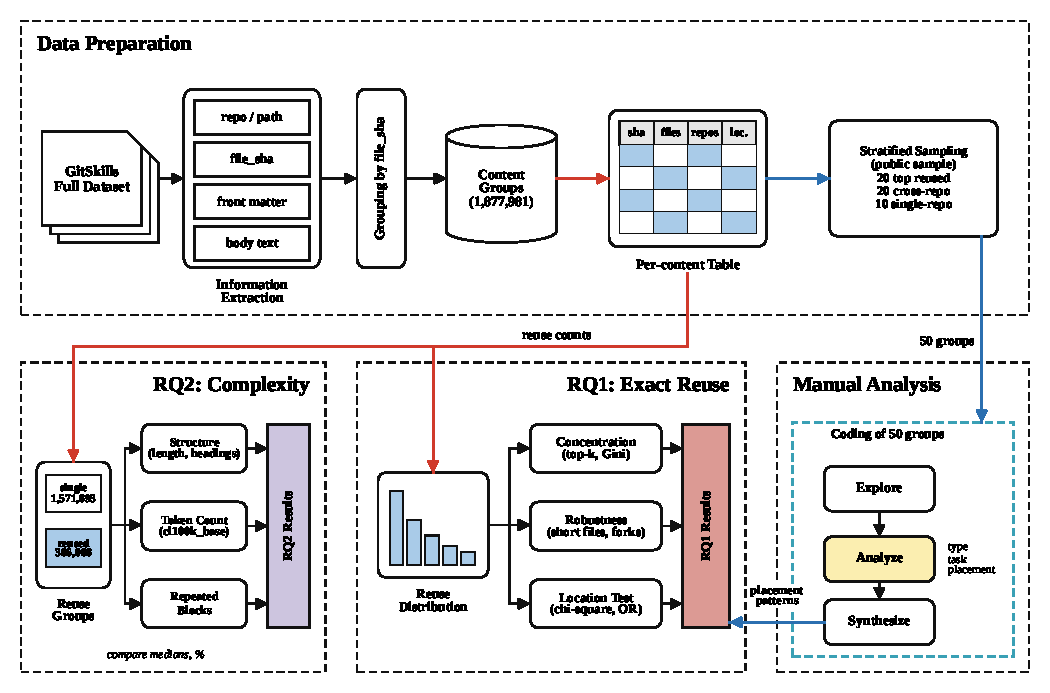
\includegraphics[width=\textwidth]{Images/approach_overview_updated.pdf}
  \caption{Overview of our approach. Data preparation groups SKILL.md files by content hash and builds a per-content table of reuse counts. RQ1 analyzes these counts. Manual analysis codes 50 sampled groups. RQ2 compares instruction length, structure, and token counts between single-repository and reused skills.}
  \label{fig:approach}
\end{figure*}

\subsection{Step 1: Dataset}
We use the full GitSkills dataset~\cite{destefanis2026gitskills} (July 2026 snapshot).
We read its Parquet release on Hugging Face\footnote{\url{https://huggingface.co/datasets/mvaccargiu/gitskills}} and download only the \texttt{artifacts} and \texttt{repos} tables.
The dataset contains 3{,}797{,}117 \texttt{SKILL.md} file occurrences of 1{,}877{,}981 distinct contents in 282{,}200 repositories.
Our counts match the numbers reported by the dataset authors, so the download is complete.
In earlier phases, we piloted the analysis on the public sample of 13{,}000 contents\footnote{\url{https://github.com/giuseppedestefanis/gitskills-sample}}.
We still use this sample for the manual analysis in Step 3.

\subsection{Step 2: Data Extraction}
From the \texttt{artifacts} table, we take the repository name, the file path, the location class, the git blob hash (\texttt{file\_sha}), whether the front matter is valid, the body length, and whether the skill folder contains scripts or reference files.
The location class is \texttt{canonical} for files in \url{.claude/skills/<name>/}, \texttt{skills-dir} for files in \url{skills/<name>/} under any other folder, and \texttt{other} for all other paths.
From the \texttt{repos} table, we take the number of stars, the fork status, and the main language.
We treat two files as exact copies when they have the same \texttt{file\_sha}, which means they are byte-for-byte identical.

\subsection{Step 3: Manual Analysis}
Before defining our metrics, we manually analyzed the data in three steps.
 
\textbf{Explore.} We read a random set of skill files and looked at the most widely reused contents, including the paths of all their copies.
 
\textbf{Analyze.} We then coded 50 content groups in a spreadsheet.
The sample includes three groups:
(A)~the 20 most widely reused contents in the sample,
(B)~20 randomly selected contents that appear in at least two repositories, and
(C)~10 randomly selected contents that appear in only one repository.
We used a fixed random seed (625) so the selection can be repeated.
For each content, we read its full text and the list of places where it appears.
We then recorded three codes:
the \emph{skill type} (general-purpose or project-specific),
the \emph{task category} (frontend, backend, devops, testing, docs, data/ML, agent-meta, domain, or other), and
the \emph{placement pattern}.
The placement patterns describe where identical contents are stored:
\emph{collection/mirror} (stored in a skill collection or mirror),
\emph{independent adoption} (stored in unrelated ordinary projects
without another identified placement pattern),
\emph{multi-agent install} (stored in the folders of several agents,
such as \texttt{.agents/}, \texttt{.claude/}, and \texttt{.codex/}),
\emph{template/scaffold} (stored in template, starter, or boilerplate
paths or repositories), and
\emph{same-owner copy} (stored mainly in repositories belonging to
the same GitHub account).
These are descriptive placement labels; they do not establish
copying direction or adoption provenance.
For contents in group C, which appear in only one repository, we recorded the type of repository that hosts them instead.
We wrote a short note for every case that was not obvious.
The definitions of all codes are in the codebook in our replication package. A second author coded the same 50 contents independently using the same codebook. We computed Cohen's $\kappa$ for each question and resolved disagreements by discussion.
 
\textbf{Synthesize.} Table~\ref{tab:manual} summarizes the results.
Three findings shaped our RQ1 metrics.
First, 19 of the 20 most reused skills in the sample are general-purpose, while 5 of the 10 single-repository skills are project-specific.
Second, among the 40 manually coded cross-repository contents in groups A and B, copies of 25 were observed in collection or mirror paths, and copies of seven were spread across many unrelated projects.
This led us to measure how concentrated reuse is.
These labels describe where copies are stored. We did not verify where the copies came from.
Third, some skills are copied into the folders of several agents, sometimes inside the same repository.
This led us to separate cross-repository reuse from duplication within one repository.
We also found very short contents (fewer than 100 characters), which are mostly symbolic-link targets such as \texttt{../.claude/SKILL.md}.
There are 145 such contents in the sample and 19{,}945 in the full dataset.
We remove them in a robustness check.
 
\begin{table}[t]
  \caption{Manual analysis of 50 content groups from the public sample. A: top-20 reused; B: random cross-repository; C: random single-repository. Inter-coder agreement (Cohen's $\kappa$): skill type 0.62, placement pattern 0.62.}
  \label{tab:manual}
  \centering
  \small
  \begin{tabular}{lrrr}
    \toprule
    & A & B & C \\
    \midrule
    \multicolumn{4}{l}{\textit{Skill type}} \\
    \quad General-purpose          & 19 & 17 & 5 \\
    \quad Project-specific         & 1  & 3  & 5 \\
    \midrule
    \multicolumn{4}{l}{\textit{Placement pattern (C: hosting repository)}} \\
    \quad Collection/mirror        & 12 & 13 & 3 \\
    \quad Independent adoption     & 5  & 2  & -- \\
    \quad Multi-agent install      & 2  & 2  & -- \\
    \quad Template/scaffold        & 1  & 1  & 4 \\
    \quad Same-owner copy          & 0  & 2  & -- \\
    \quad None recorded            & -- & -- & 3 \\
    \midrule
    Total                          & 20 & 20 & 10 \\
    \bottomrule
  \end{tabular}
\end{table}
 
\subsection{Step 4a: RQ1 Measurement}
\begin{figure}[t]
  \centering
  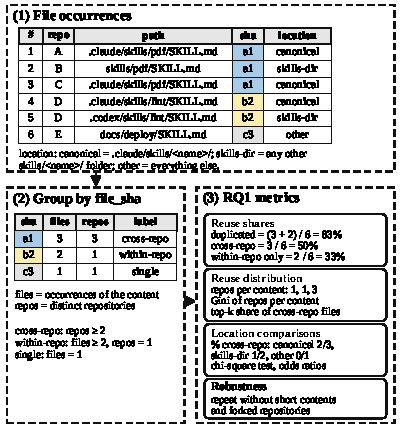
\includegraphics[width=\columnwidth]{Images/rq1_whitebox.pdf}
  \caption{White-box view of RQ1 on a toy example with six files. (1) Each file has a content hash and a location class. (2) Files are grouped by hash, and each content is labeled by its number of files and repositories. (3) The RQ1 metrics are computed from these groups.}
  \Description{Three panels: a table of six files, a table of three content groups, and boxes with the RQ1 metrics.}
  \label{fig:rq1-whitebox}
\end{figure}


We group all occurrences by \texttt{file\_sha}.
For each distinct content, we count how many times it occurs and in how many different repositories.
Based on these counts, we report:
\begin{enumerate}
  \item the share of occurrences that are \emph{duplicated} (the content appears more than once), \emph{cross-repository} (the content appears in two or more repositories), or \emph{within-repository only};
  \item the distribution of contents and occurrences over the number of repositories;
  \item the concentration of reuse, using the share held by the top-$k$ contents and the Gini coefficient;
  \item two robustness checks, removing very short contents and removing forked repositories; and
  \item whether reuse differs by location class, using a chi-square test, Cram\'er's $V$, and odds ratios with 95\% confidence intervals.
\end{enumerate}
All queries are written in DuckDB in one script (\texttt{code/rq1\_reuse.py}), which is part of our replication package.

Figure~\ref{fig:rq1-whitebox} shows these steps on a small example.
Content \texttt{a1} appears in three repositories, so its three files are cross-repository.
Content \texttt{b2} has two copies in the same repository, so its files are within-repository only.
Content \texttt{c3} has only one file.
In this example, 5 of the 6 files are duplicated (83\%) and 3 of the 6 are cross-repository (50\%).

\subsection{Step 4b: RQ2 Measurement}

For our RQ2, we extend our preliminary analysis to the full
GitSkills dataset described in Step 1. We analyze each distinct
\texttt{SKILL.md} content once and compare skills used in one
repository with those reused across multiple repositories.
The full dataset contains 1{,}571{,}893 single-repository
contents and 306{,}088 cross-repository contents.

We use DuckDB to read the Parquet files from the
\texttt{artifacts} table. We group file occurrences by
\texttt{file\_sha} and count distinct \texttt{repo\_full\_name}
values to determine repository coverage. We select one
representative per distinct content using
\texttt{dedup\_primary = 1}. Contents found in at least
two repositories are classified as reused.

Figure~\ref{fig:rq2-whitebox} illustrates the internal
steps of our RQ2 measurements, including data preparation,
instruction processing, feature extraction, and aggregation.

\begin{figure*}[t]
    \centering
    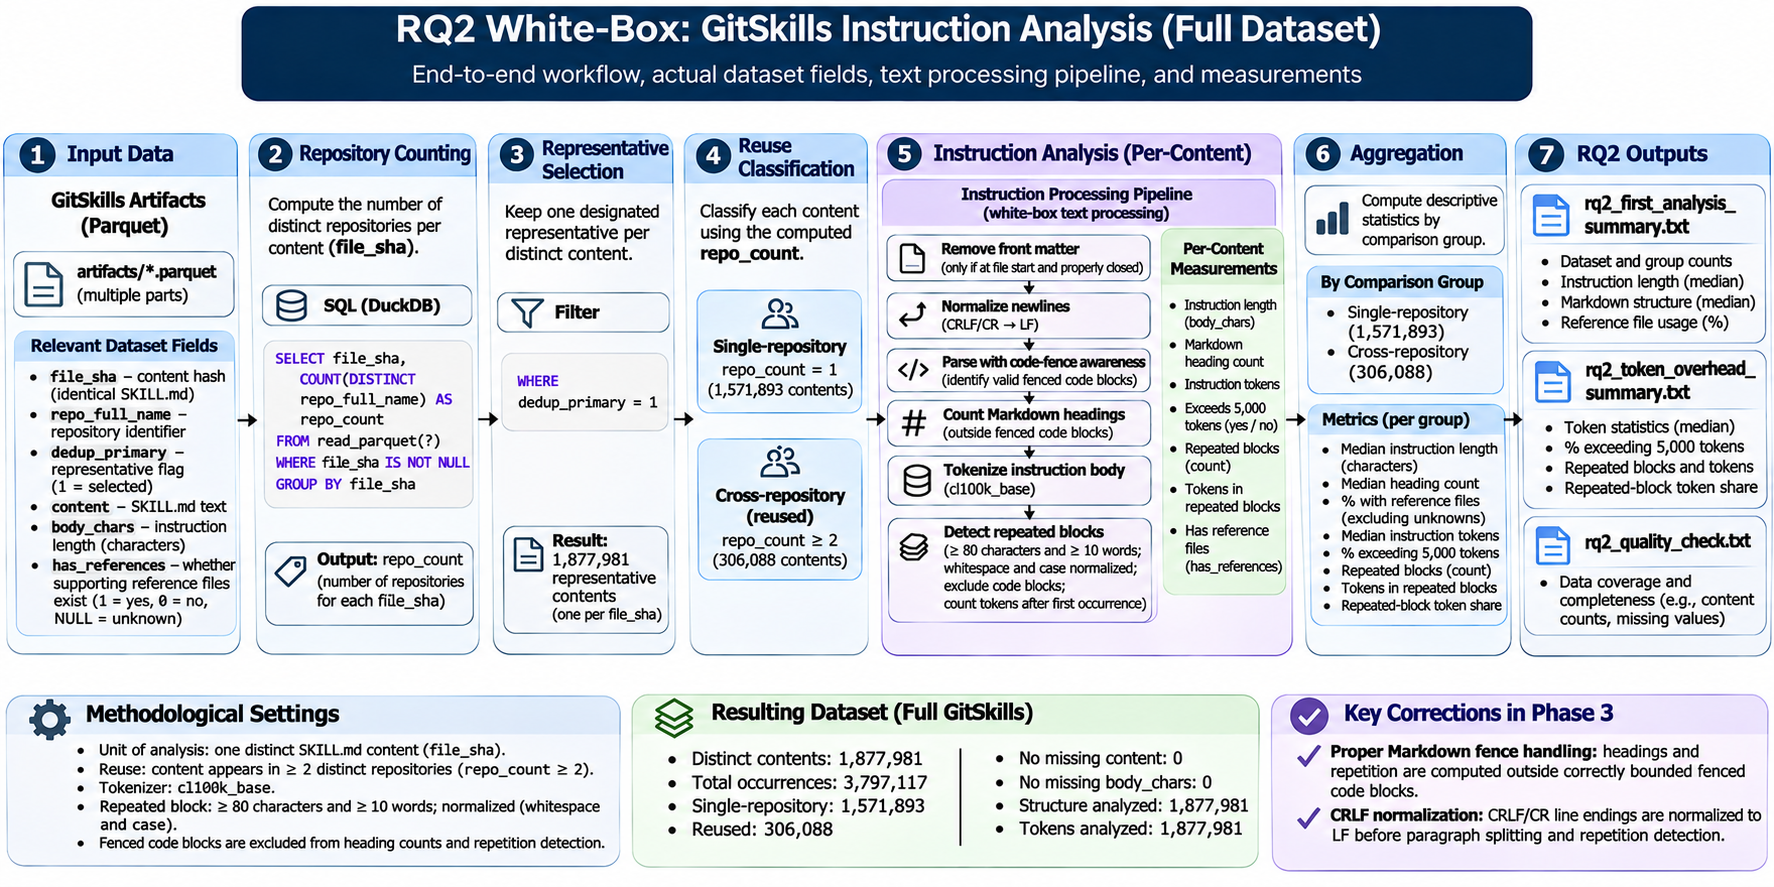
\includegraphics[width=\textwidth]{Images/rq2_whitebox.png}
    \caption{White-box view of the RQ2 analysis using the full
    GitSkills dataset. File occurrences are grouped by content
    hash, and one representative is selected per distinct
    content. Instruction length, Markdown headings, reference
    files, token counts, and repeated blocks are measured and
    compared between single-repository and reused skills.}
    \Description{Seven-stage workflow showing GitSkills Parquet
    input, repository counting, representative selection, reuse
    classification, instruction processing, aggregation, and
    RQ2 output summaries.}
    \label{fig:rq2-whitebox}
\end{figure*}

First, we examine instruction length, Markdown headings,
and the presence of supporting reference files to understand
how the instructions are organized and how detailed they are.
Instruction length is measured using \texttt{body\_chars},
while reference-file presence is obtained from
\texttt{has\_references}. Unknown reference values are
excluded when calculating percentages.

Markdown headings are counted outside fenced code blocks.
We corrected the parser to track the opening fence character
and length, requiring a valid closing fence with the same
character and at least the opening length.

Second, we use Python and the \texttt{cl100k\_base} tokenizer
to measure instruction-token counts after removing valid
leading YAML front matter. We also identify skills exceeding
5{,}000 tokens and detect repeated instruction blocks within
individual files.

Before paragraph segmentation, we normalize CRLF and CR
line endings to LF. We compare paragraphs after normalizing
whitespace and letter case, considering blocks with at least
80 characters and 10 words. Fenced code blocks are excluded
from repetition detection. Repeated-token counts exclude
the first occurrence of each matching block.

We added regression tests for newline normalization and
Markdown fence handling. The final replication package contains 21 passing tests covering parsing, the full-data pipeline, and example auditing. Re-running the corrected analysis on the preliminary sample preserved
the reported aggregate results.

\section{Experiments}
\label{Section:Result}

\subsection{RQ1: How is exact SKILL.md reuse distributed across repositories?}
\textbf{Motivation.}
GitSkills reports that about half of all skill files are exact copies.
However, it does not show how this reuse is spread.
If most copies come from a few popular skills, the dataset is less diverse than its size suggests.
If copies are spread out, most skills are written for their own repository.

\textbf{Approach.}
We apply the measurements from Step 4a to all 3{,}797{,}117 occurrences.

\begin{table}[t]
  \caption{Exact reuse of SKILL.md files in the GitSkills dataset.}
  \label{tab:rq1-overview}
  \centering
  \small
  \begin{tabular}{lrr}
    \toprule
    Metric & All files & Body $\geq$ 100 chars \\
    \midrule
    File occurrences                      & 3{,}797{,}117 & 3{,}745{,}469 \\
    Distinct contents                     & 1{,}877{,}981 & 1{,}858{,}036 \\
    Contents in $\geq$2 repositories      & 306{,}088     & 303{,}013 \\
    \% occurrences duplicated             & 60.77\%        & 60.65\% \\
    \% occurrences cross-repository       & 54.91\%        & 54.87\% \\
    \% occurrences within-repository only & 5.86\%         & 5.78\% \\
    \bottomrule
  \end{tabular}
\end{table}

\textbf{Results.}
\emph{Reuse is common, and most of it is across repositories.}
Table~\ref{tab:rq1-overview} shows that 60.8\% of all files share their exact content with at least one other file.
Also, 54.9\% of all files have a content that appears in two or more repositories.
Only 5.9\% of files are duplicates within a single repository.
These within-repository duplicates belong to 82{,}413 contents.
In 67.2\% of them, the copies are in different top-level folders, which fits the multi-agent install pattern from our manual analysis.
Our ``duplicated'' share counts every file in a duplicated group.
GitSkills reports 50.5\%, but it does not count the first file of each group.
With that definition, we get $(3{,}797{,}117-1{,}877{,}981)/3{,}797{,}117 = 50.5\%$, which matches the GitSkills paper.

\begin{figure}[t]
  \centering
  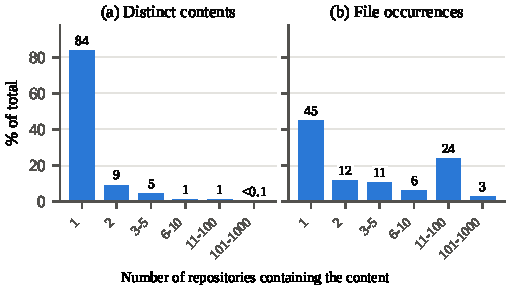
\includegraphics[width=\columnwidth]{Images/rq1_repos_per_content.pdf}
  \caption{Number of repositories that contain each distinct content, as a share of (a)~distinct contents and (b)~file occurrences.}
  \label{fig:rq1-dist}
\end{figure}

\emph{Most skills are unique, but most files are copies.}
Figure~\ref{fig:rq1-dist} shows both sides.
Most distinct contents (83.7\%, or 1{,}571{,}893) appear in only one repository.
Only 1.3\% (23{,}475 contents) appear in more than ten repositories.
When we count files instead of contents, the picture changes.
Single-repository contents make up only 45.1\% of all files.
The 23{,}475 contents found in more than ten repositories make up 26.8\%.
The Gini coefficient of repositories per content is 0.38.

\begin{figure}[t]
  \centering
  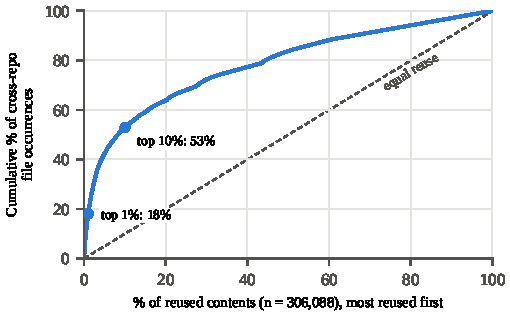
\includegraphics[width=\columnwidth]{Images/rq1_concentration.pdf}
  \caption{Concentration of cross-repository reuse. Contents found in at least two repositories are sorted from most to least reused. The line shows their cumulative share of cross-repository file occurrences. The dashed line shows equal reuse.}
  \label{fig:rq1-conc}
\end{figure}

\emph{Reuse has a clear head but a long tail.}
There are 306{,}088 contents that appear in at least two repositories.
The top 1\% of them (about 3{,}000 contents) account for 18.1\% of all cross-repository occurrences.
The top 10\% account for 52.9\% (Figure~\ref{fig:rq1-conc}).
The 100 most reused contents account for only 2.1\%.
In our pilot sample, the top 100 held 30.7\%.
The sample has only 2{,}854 reused contents, so a few popular skills had much more weight there.
The most reused skills are general-purpose guides, not project instructions.
Examples are \texttt{frontend-design} (951 repositories), \texttt{verification-before-completion} (914), \texttt{webapp-testing} (781), \texttt{pdf} (661), and \texttt{systematic-debugging} (656).
This matches our manual analysis, where 19 of the 20 most reused skills in the sample were general-purpose.
Copies of the 100 most reused contents are not more often in collection or mirror paths than the average file (3.4\% vs.\ 5.4\%).

\emph{Robustness.}
Our results stay the same after removing very short contents (54.9\% cross-repository in both cases).
They also stay the same after removing forked repositories (54.8\%).
The dataset contains almost no forks, because GitHub code search indexes very few of them.

\emph{Location.}
Table~\ref{tab:rq1-location} shows that cross-repository reuse is linked to where a file is stored.
However, the direction depends on what we count.
When we count every file, files in \texttt{.claude/skills/} are the least often shared (42.8\% vs.\ 57.2\% for files in the ``other'' class; OR $= 0.56$; $\chi^2(2)=25{,}503$, $p<0.001$).
When we count each distinct content once, the result is the opposite.
Contents stored in \texttt{.claude/skills/} are reused more often (23.5\% vs.\ 11.3\%; OR $= 2.42$; $\chi^2(2)=21{,}538$, $p<0.001$).
Heavily copied contents have many copies outside \texttt{skills/} folders, which raises the file-level share for the ``other'' location.
The observed location differences are statistically significant,
so we also examine effect sizes.
Both effects are small (Cram\'er's $V = 0.08$ and $0.11$).
The file-level test also treats copies of the same content as independent, so its $p$-value is too optimistic.
For this reason, we rely more on the content-level result.

\begin{table}[t]
  \caption{Location vs.\ cross-repository reuse. Odds ratios (OR) are relative to files in the ``other'' location class. All $p<0.001$ (chi-square test).}
  \label{tab:rq1-location}
  \centering
  \small
  \begin{tabular}{llrrr}
    \toprule
    Unit & Location & $n$ & \% cross-repo & OR [95\% CI] \\
    \midrule
    Files    & canonical  & 373{,}652     & 42.8 & 0.56 [0.55, 0.56] \\
             & skills-dir & 2{,}102{,}053 & 55.6 & 0.94 [0.93, 0.94] \\
             & other      & 1{,}321{,}412 & 57.2 & 1.00 (ref.) \\
    \midrule
    Contents & canonical  & 273{,}721     & 23.5 & 2.42 [2.39, 2.45] \\
             & skills-dir & 1{,}037{,}938 & 17.1 & 1.63 [1.61, 1.65] \\
             & other      & 566{,}322     & 11.3 & 1.00 (ref.) \\
    \bottomrule
  \end{tabular}
\end{table}

\textbf{Examples.}
We count a content as reused when the same file hash appears in two or more repositories.
Three cases from the data show where this works and where it fails.
\begin{itemize}
\item \textbf{True positive.} \texttt{frontend-design} has exactly the same bytes in 951 repositories.
This is the exact cross-repository reuse that RQ1 measures.
\item \textbf{False positive.} One ``skill'' in the public sample contains only the line \url{../../../agents/product/cs-agile-product-owner.md}.
It appears in 28 repositories, so it counts as reuse.
However, it is the text of a symbolic link, not an instruction file.
Our robustness check removes such short contents.
\item \textbf{False negative.} \texttt{shadcn} appears unchanged in 132 repositories of the sample.
One more repository has the same skill with two front-matter lines removed (\texttt{user-invocable} and \texttt{allowed-tools}).
The hash changes, so this copy counts as a separate content found in only one repository.
\end{itemize}
Exact hashing is reliable for identical copies but misses edited ones.
So the real amount of reuse is likely higher than our numbers show.

\textbf{Summary of RQ1.}
About 61\% of \texttt{SKILL.md} files are exact copies, and most of this reuse happens across repositories.
At the same time, 84\% of distinct skill contents occur in only one repository.
Reuse has a clear head but a long tail: the top 10\% of reused contents account for about half of cross-repository occurrences.
The most reused skills are general-purpose guides.
Skills stored in standard \texttt{skills/} folders are more likely to be reused than skills stored elsewhere, but the effect is small.
\subsection{RQ2: How do instruction characteristics differ
between single-repository and cross-repository skill contents?}

\textbf{Motivation.}
As discussed in our problem statement, authors must choose
between concise instructions and broader coverage of repository
requirements. Longer or more detailed instructions may increase
the amount of text that AI agents need to process. In this study,
we examine how instruction length and structure relate to
potential input-token overhead using the full GitSkills dataset.

\textbf{Approach.}
We apply the measurements from Step 4b to the full GitSkills
dataset. We compare 1{,}571{,}893 distinct contents found in one
repository with 306{,}088 contents reused across multiple
repositories. We examine instruction length, Markdown headings,
supporting reference files, and token counts. We also identify
repeated instruction blocks within individual files.

\begin{table}[t]
    \caption{RQ2 results comparing single-repository
    and reused SKILL.md contents in the full GitSkills dataset.}
    \label{tab:rq2-results}
    \centering
    \footnotesize
    \setlength{\tabcolsep}{3pt}
    \begin{tabular}{@{}p{0.48\columnwidth}rr@{}}
        \toprule
        Metric & Single repo & Reused \\
        \midrule
        Distinct contents & 1,571,893 & 306,088 \\
        Median length (chars) & 4,548 & 4,903 \\
        Median headings & 11 & 12 \\
        With reference files & 25.8\% & 26.5\% \\
        Median tokens & 1,206 & 1,257 \\
        Over 5,000 tokens & 5.8\% & 6.1\% \\
        With repeated blocks & 0.7\% & 0.6\% \\
        Repeated token share & 0.08\% & 0.07\% \\
        \bottomrule
    \end{tabular}
\end{table}

\textbf{Results.}
\emph{Reused skills have slightly longer instructions and
somewhat higher token counts.}
Table~\ref{tab:rq2-results} shows that reused skills have a
median instruction length of 4,903 characters, compared with
4,548 for single-repository skills. Reused skills also have
more Markdown headings, with a median of 12 compared with 11.
The median token counts are 1,257 and 1,206 tokens,
respectively. Although reused skills have higher median
token counts, the difference is relatively small at 51 tokens.
These measurements describe instruction size rather than
actual agent execution costs.

\emph{Supporting reference files are slightly more common
among reused skills.}
We found that 26.5\% of reused skills have supporting reference
files, compared with 25.8\% of single-repository skills.
This differs from our preliminary sample, where supporting
reference files were less common among reused skills.
The full-dataset difference is small, suggesting that
reference-file presence is broadly similar between the two
groups. However, these measurements use the primary
occurrence of each distinct content, and reference-file
availability may differ across copies.

\emph{Exact repeated instruction blocks are uncommon.}
Across all 1{,}877{,}981 distinct contents, 5.8\% exceed 5,000
instruction tokens. We also found that only 0.7\% of skills
contain repeated instruction blocks under our detection
criteria. In total, we identified 49{,}179 repeated blocks
containing 2{,}823{,}988 tokens. These account for approximately
0.08\% of the total instruction tokens.

Single-repository skills have a repeated-token share of
0.08\%, compared with 0.07\% for reused skills. Although
the full dataset contains many more repeated blocks than
the preliminary sample, their overall token share remains
approximately the same. This suggests that exact paragraph
repetition contributes little to the overall instruction size.
However, our method does not detect similar instructions
written in different words.


\textbf{Examples.}
We manually reviewed four skill files to check how well our
repetition detector worked. In two files from
\texttt{RakhilML/ReBrowse}, related to Stack Overflow and
Wikipedia APIs, we found the same Markdown table under two
different GET endpoints. Our detector identified one repeated
block containing 32 tokens in each file. As the repeated tables
were correctly identified, we labeled both cases as true
positives.

In the DevOps skill from \texttt{nicobit/spec-poc}, we found
the same YAML metadata repeated twice. The earlier exploratory
detector counted it as repetition. However, our corrected
detector excluded the first YAML front-matter block and found
no repeated blocks. We labeled this as a false positive of
the exploratory detector, not the corrected detector.

In the Senior UX Designer skill from \texttt{wk23aau/xapply},
we found the same five capabilities listed under both
Capabilities and System Prompt. However, our corrected detector
reported zero repeated blocks because these lists appeared
within different paragraphs. We labeled this as a false
negative based on our manual review. This shows that our method
can miss repeated content when it appears in different paragraph
structures.

These examples also show that repeated content is not always
unnecessary, since the same information may be useful in
different sections or endpoints.


\textbf{Summary of RQ2.}
Our full-dataset results show that reused skills have slightly
higher instruction-token requirements than single-repository
skills, although the difference in median tokens remains
relatively small. Some differences also exist in their length
and structure. Exact paragraph repetition is uncommon, while
a small proportion of skills contain particularly long
instructions. These findings provide a descriptive
understanding of potential input-token overhead.
Further experiments are needed to determine whether these
characteristics affect actual AI agent efficiency.

\label{Section:Discussion}

\section{Threats To Validity}
\label{Section:Threats}
\subsection{Conclusion Validity}
\textit{RQ1.}
The large sample makes small location differences statistically
detectable.
The file-level chi-square test also treats copies of the same content as independent, so its p-value is too optimistic.
For this reason, we report effect sizes (Cram\'er's $V$ and odds ratios) and rely more on the content-level test.
The manual analysis covers only 50 contents, so its counts cannot be generalized to the whole dataset.


\textit{RQ2.}
The way we analyzed RQ2 was by comparing instruction
characteristics using medians, percentages, and token counts.
We found that the differences between single-repository
and cross-repository skills were generally small, even
though we used the full dataset. We did not run statistical
significance tests or examine other factors that might
affect instruction length. We also manually checked four selected skill files to
understand where our repetition detector worked and where
it missed repeated content. Since these examples were
selected for inspection rather than randomly sampled,
we cannot use them to measure the detector's overall
accuracy.
Therefore, our results show differences between the two
groups, but we cannot make strong claims about the
relationship between repository reuse and instruction
complexity.

\subsection{Internal Validity}
\textit{RQ1.}
Our results describe where copies are stored, not why they were copied.
We do not claim that location causes reuse.
For the content-level location test, each content is assigned to the location of its representative file (\texttt{dedup\_primary}), although its copies may be stored in other locations.
The manual codes involve judgment.
To reduce this threat, two authors coded the 50 contents independently (Cohen's $\kappa$ from 0.62 to 0.91) and resolved disagreements by discussion.


\textit{RQ2.}
Our RQ2 results depend on how we process and measure
the skill files. Different line endings, Markdown code
fences, and YAML front matter can affect the measurements.
To reduce these errors, we corrected the parsing code
and ran the 21 tests included in the final replication package. We also manually checked four skill files to examine the repetition detector.
Some unusual file structures may still affect the results.
Our analysis compares instruction characteristics between
the two groups, but it does not show that repository reuse
causes differences in instruction length or token counts.


\subsection{Construct Validity}
\textit{RQ1.}
We measure reuse with exact content hashes.
This misses near-duplicates: a copy with one changed line counts as a different content (see the false negative in Section~6.1).
It also counts some files as reuse that are not real skills, such as one-line relative paths left by symbolic links (the false positive in Section~6.1).
We remove the 19{,}945 contents with fewer than 100 characters in a robustness check, and the cross-repository share stays at 54.9\%.


\textit{RQ2.}
For RQ2, we measure reuse using exact content hashes.
This shows whether the same content appears in multiple
repositories, but not why it was copied. We estimate
instruction tokens using the \texttt{cl100k\_base} tokenizer,
so the counts may differ for other models. Our repetition
detector only finds matching paragraph blocks. It may miss
repeated lists in different paragraphs or instructions
written in different words. Therefore, our results measure
instruction characteristics, not the actual cost of
running AI agents.

\subsection{External Validity}
\textit{RQ1.}
GitSkills only covers public GitHub repositories found by GitHub code search, in a July 2026 snapshot.
Skills in private projects or on other platforms may be reused differently.
Code search indexes very few forks, so reuse through forking is mostly missing.
The manual analysis uses the public sample, so its 50 contents are not the most reused contents of the full dataset.


\textit{RQ2.}
Our analysis uses the full GitSkills dataset rather than
the preliminary sample. However, GitSkills only covers
public GitHub repositories found through code search.
Skills from private repositories or other platforms are
not included. The results also reflect the July 2026
snapshot, so they may change as skills are updated or
new repositories are added. Our findings describe the
skills available in this dataset and may not apply to
all agent skills.

% For RQ2, token counts depend on the selected
% \texttt{cl100k\_base} tokenizer and the handling of front
% matter. Heading and repeated-block detection use heuristics
% rather than complete semantic analysis. The 5,000-token
% threshold is a descriptive cutoff, not a model capacity
% limit. Repeated text may serve a useful purpose, and its
% token share does not establish achievable savings from
% removing it. These analyses do not measure agent runtime,
% task success, or causal effects of instruction design.

\section{Conclusion}
\label{Section:Conclusion}
Our analysis shows that exact cross-repository reuse accounts for a substantial share of file occurrences in the GitSkills dataset. Reuse has a clear head but a long tail: the top 10\% of reused contents account for about half of cross-repository occurrences.

We compared 1,571,893 single-repository contents with
306,088 cross-repository contents. Reused skills have
slightly longer instructions and more Markdown headings.
The median token counts are 1,206 for single-repository
skills and 1,257 for reused skills, a difference of only
51 tokens.

Repeated instruction blocks are uncommon. Only about
0.7\% of skills contain repeated blocks, accounting for
approximately 0.08\% of instruction-body tokens. Our
method may still miss repeated lists in different paragraph
structures or instructions written in different words.
These results describe instruction characteristics in
GitSkills, but do not show whether they affect actual
AI agent performance.

\section{Future Work}
\label{Section:FutureWork}
Future work could examine skills with similar instructions
that are not exact copies. Additionally, we could conduct
a larger manual review with qualitative analysis to better
understand instruction patterns and compare token counts
using different tokenizers. Moreover, we could run controlled
experiments to examine whether instruction length, structure,
or repetition affects AI agent runtime, actual token usage,
and task success.

\section*{Acknowledgment of AI Assistance}
ChatGPT assisted with drafting the RQ2 text from the analysis
results and preparing its white-box illustration. Claude assisted
with revising results prose and preparing the related-work table.
Codex assisted with final editing, package integration,
documentation, and verification checks. These tools were used
as aids; the authors remain responsible for the reported methods,
evidence, interpretations, and final submission.

\section*{Replication Materials}
Our analysis scripts, result summaries, and instructions
for obtaining the dataset and reproducing the experiments
are available at:
\url{https://github.com/Rymarmar/ssw625-group6-gitskills}

% \bibliographystyle{ACM-Reference-Format}
\bibliographystyle{unsrt}
\bibliography{sample-base}


\end{document}
\endinput
%%
%% End of file `sample-authordraft.tex'.
